\documentclass[oneside, a4paper]{memoir}

\usepackage{supertabular}
\usepackage[sc]{mathpazo}
\usepackage[hmarginratio=1:1,margin=1in]{geometry}
\usepackage{fancyhdr}
  % Creates footer
  \pagestyle{fancy}%
  \fancyhf{}%
  \lfoot{Assignment}
  \cfoot{\emph{Swapnil}}
  \rfoot{Index}
  \renewcommand{\headrulewidth}{0pt}% Line at the head invisible
  \renewcommand{\footrulewidth}{2pt}% Line at the footer visible
\usepackage{tcolorbox}
\usepackage{graphicx}
\usepackage{multirow}
  \graphicspath{ {./images/} }

\usepackage{enumitem}
  \setlist[enumerate]{noitemsep}



\begin{document}
\begin{tcolorbox}
  \Huge
  \centering
  \textsc{Table of Content}
\end{tcolorbox}
\noindent\resizebox{\columnwidth}{!}{
  \begin{supertabular}{rp{8cm}crl}
      & \textbf{Name of experiment} & \textbf{Date of experiment} & \textbf{Page no.} & \textbf{Signature}\\
      \cmidrule{2-5}
      1 &
        Write a program in HTML of the following:
        \begin{enumerate}
          \item To insert two image files.
          \item To use hyperlink to connect two pages.
          \item To insert three headings of different sizes.
        \end{enumerate}&
        07-11-2022 &
        1-2 &
        \multirow{17}{*}{}\\
      \cmidrule{1-4}
      2 &
        Write a program in HTML to display the following table 

        \vskip8pt
        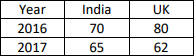
\includegraphics[scale=0.7]{3} &
        07-11-2022 &
        3 \\
      \cmidrule{1-4}
      3 &
        Write a program in JavaScript to multiply two numbers using two text boxes, one command button and on-click event handler &
        07-11-2022 &
        4-5 \\
      \cmidrule{1-4}
      4 &
        Write a HTML program to input name, roll no, semester, department \& year of a student and display the output in a tabular form. &
        08-11-2022 &
        6-7 \\
      \cmidrule{1-4}
      5 &
        Write a program to design a database of a student with attributesname, roll no, contact no, DOB, department, year in XML. &
        10-11-2022 &
        8-10 \\
      \cmidrule{1-4}
      6 &
        Write a JavaScript program to display a character string in the reverse order. &
        10-11-2022 &
        11-12 \\
      \cmidrule{1-4}
      7 &
        Write a JavaScript code to count the number of digits in a given number. &
        14-11-2022 &
        13 \\
      \cmidrule{1-4}
      8 &
        Write a HTML to design a form that has the following attribute Name, Address, E-mail, Contact Number. &
        14-11-2022 &
        14-15 \\
      \cmidrule{1-4}
      9 &
        Write a code in HTML to
        \begin{enumerate}
          \item Layout pages using tables;
          \item Create navigation bars;
        \end{enumerate}&
        25-11-2022 &
        16-18 \\
      \cmidrule{1-4}
      10 &
        Write a JavaScript code to pick a phrase from an array of sent. &
        25-11-2022 &
        19 \\
      \cmidrule{1-4}
      11 &
        Write a JavaScript to show event on button and list. &
        28-11-2022 &
        20 \\
      \cmidrule{1-4}
      12 &
        Write a program that prints a table of numbers from 5 to 15 and their squares and cubes using alert. &
        28-11-2022 &
        21-22 \\
      \cmidrule{1-4}
      13 &
        Write a program that prints the largest of three number. &
        01-12-2022 &
        23-24 \\
      \cmidrule{1-4}
      14 &
        Write a program that finds the factorial of a number n. &
        01-12-2022 &
        25-26 \\
      \cmidrule{1-4}
      15 &
        Enter a list of positive numbers terminated by Zero. Find the sum and average of these numbers. &
        01-12-2022 &
        27-28 \\
      \cmidrule{1-4}
      16 &
        A person deposits Rs 1000 in a fixed account yielding 5\% interest. Compute the amount in the account at the end of each year for n years &
        14-12-2022 &
        29-30 \\
      \cmidrule{1-4}
      17 &
        Read n numbers. Count the number of negative numbers, positive numbers and zeros in the list. &
        14-12-2022 &
        31-32 \\
    \end{supertabular}
  }

\end{document}
